%%%%%%%%%%%%%%%%%%%%%%%%%%%%%%%%%%%%%%%%%%%%%%%%
%% Compile: XeLaTeX BibTeX XeLaTeX XeLaTeX
%% Course Slides: LaTeX 4 Linguists -- LOT 2019, Amsterdam
%% Antonio Machicao y Priemer
%%%%%%%%%%%%%%%%%%%%%%%%%%%%%%%%%%%%%%%%%%%%%%%%

%\documentclass[a4paper,10pt, bibtotoc]{beamer}
\documentclass[a4paper,10pt,handout]{beamer}

%%%%%%%%%%%%%%%%%%%%%%%%%
%% PACKAGES & COMMANDS 
%%%%%%%%%%%%%%%%%%%%%%%%%

%%%%%%%%%%%%%%%%%%%%%%%%%%%%%%%%%%%%%%%%%%%%%%%%%%%%
%%%          MyP-Packages   2018.12.08    XeLaTeX
%%%%%%%%%%%%%%%%%%%%%%%%%%%%%%%%%%%%%%%%%%%%%%%%%%%%


%\usepackage[utf8]{inputenc} %XeLaTeX

%% For German texts
\usepackage[ngerman,english]{babel}

%% For English texts
%\usepackage[ngerman,english]{babel}

%% Captions numbered in Beamer 
\setbeamertemplate{caption}[numbered]

%% Change ''Abbildung'' into ''Abb.'' 
%% for: babel
	\renewcommand{\thefigure}{\arabic{figure}}
	\addto\captionsngerman{%
		\renewcommand{\figurename}{Abb.}%
	}
	\renewcommand{\figurename}{Abb.} 

%% Change ''Figure'' into ''Fig.'' 
%% for: babel
	\renewcommand{\thefigure}{\arabic{figure}}
	\addto\captionsenglish{%
		\renewcommand{\figurename}{Fig.}%
	}
%	\renewcommand{\figurename}{Fig.} %% << not needed? 


%% TIPA encoding needs options: T3 & T1
\usepackage[T3,T1]{fontenc}  %not needed in XeLaTeX (?)

%\usepackage{fontspec} % XeLaTeX: Problem: Libertine+Fontspec+TIPA

%% Font
\usepackage{lmodern}
%\usepackage{libertine} % XeLaTeX: Problem: Libertine+Fontspec+TIPA

%% Blind text: \blindtext \Blindtext \blindtext[5] \blindlist{itemize}[x] ...
\usepackage{blindtext}

%% ulem: Strike out
\usepackage[normalem]{ulem}  

%% graphicx: if gb4e is active PDFLaTeX does not accept files with underline. PDFLaTeX accepts files only with .jpg, .png, .pdf endings
\usepackage{graphicx}

%% Math symbols
\usepackage{amsmath}
\usepackage{amsfonts}
\usepackage{amssymb}
\usepackage{MnSymbol} 				% Meaning brackets 

%% Toggles
\usepackage{etoolbox}
	\newtoggle{handout}


%%%%%%%%%%%%%%%%%%%%%%%%%%%%%%%%%%%%%%%%%%%%%%%%%%%%
%%%         Tables & Lists & Columns            
%%%%%%%%%%%%%%%%%%%%%%%%%%%%%%%%%%%%%%%%%%%%%%%%%%%%

% Text in columns: \begin{multicols}{n} \columnbreak \end{multicols}
\usepackage{multicol}
%	\setlength{\columnsep}{.5cm}	

%% Tables with specified width
\usepackage{tabularx}

%% For complex tables
\usepackage{array}

%% For other tables
\usepackage{booktabs}

%% For more than one row in a table
\usepackage{multirow}

%% Special lists: itemize*
\usepackage{mdwlist}


%%%%%%%%%%%%%%%%%%%%%%%%%%%%%%%%%%%%%%%%%%%%%%%%%%%%
%%%          Coloured elements                  
%%%%%%%%%%%%%%%%%%%%%%%%%%%%%%%%%%%%%%%%%%%%%%%%%%%%
%Use xcolor before `gb4e'!
\usepackage{xcolor}


%%%%%%%%%%%%%%%%%%%%%%%%%%%%%%%%%%%%%%%%%%%%%%%%%%%%
%%%          Trees                               
%%%%%%%%%%%%%%%%%%%%%%%%%%%%%%%%%%%%%%%%%%%%%%%%%%%%
%% Forest must be loaded before `gb4e'
\usepackage{forest}
	
	%% Needed for the "actual forest version"
	\useforestlibrary{linguistics}
	\forestapplylibrarydefaults{linguistics}

%% Old forest version
%\usepackage{etex}		%For Forest bug
%\usepackage{../forestold}
	
	
%%%%%%%%%%%%%%%%%%%%%%%%%%%%%%%%%%%%%%%%%%%%%%%%%%%%
%%%          Venndiagram                         
%%%%%%%%%%%%%%%%%%%%%%%%%%%%%%%%%%%%%%%%%%%%%%%%%%%%
%% Package needed: tikz
\usepackage{venndiagram}


%%%%%%%%%%%%%%%%%%%%%%%%%%%%%%%%%%%%%%%%%%%%%%%%%%%%%
%%%%          Verbatim                            
%%%%%%%%%%%%%%%%%%%%%%%%%%%%%%%%%%%%%%%%%%%%%%%%%%%%%
%%`Listings' must be loaded before `gb4', use `verbatim' otherwise
\usepackage{listings}

\lstset{
	language=TeX,
	backgroundcolor=\color{lightgray},
	basicstyle={\footnotesize\ttfamily\color{blue}},
	showstringspaces=false,
	columns=flexible
}
\lstset{literate=%
	{Ö}{{\"O}}1
	{Ä}{{\"A}}1
	{Ü}{{\"U}}1
	{ß}{{\ss}}2
	{ü}{{\"u}}1
	{ä}{{\"a}}1
	{ö}{{\"o}}1
}

%\lstset{%frame=tb,
%	language=Perl,
%	aboveskip=3mm,
%	belowskip=3mm,
%	showstringspaces=false,
%	columns=flexible,
%	basicstyle={\small\ttfamily\color{blue}},
%	numbers=none,
%	%numberstyle=\tiny\color{gray},
%	extendedchars=false,
%	morekeywords={foo},
%	otherkeywords={\#\#},
%	%keywordstyle=\color{blau},
%	%commentstyle=\color{whiteblue},
%	%stringstyle=\color{mauve},
%	breaklines=true,
%	breakatwhitespace=true,
%	tabsize=3
%}


%%%%%%%%%%%%%%%%%%%%%%%%%%%%%%%%%%%%%%%%%%%%%%%%%%%%%
%%%%       Attribute Value Matrices               
%%%%%%%%%%%%%%%%%%%%%%%%%%%%%%%%%%%%%%%%%%%%%%%%%%%%%
\usepackage{../../texfiles-beamer/avm}
%%% Setting of avm (see LSP Guidelines)
	%	\avmfont{\sc}
	%	\avmvalfont{\it}
	\avmfont{\normalfont \scshape} 
	\avmvalfont{\normalfont \itshape} 
%% command to fontify the type values of an avm 
	\newcommand{\tpv}[1]{{\avmjvalfont #1}} 
%% command to fontify the type of an avm and avmspan it
	\newcommand{\tp}[1]{\avmspan{\tpv{#1}}}


%%%%%%%%%%%%%%%%%%%%%%%%%%%%%%%%%%%%%%%%%%%%%%%%%%%%
%%%          IPA                                 
%%%%%%%%%%%%%%%%%%%%%%%%%%%%%%%%%%%%%%%%%%%%%%%%%%%%
%\usepackage[noenc,safe]{tipa}	%in PDFLaTeX
\usepackage[safe]{tipa}	% in XeLaTeX


%%%%%%%%%%%%%%%%%%%%%%%%%%%%%%%%%%%%%%%%%%%%%%%%%%%%
%%%          Vowel diagram                       
%%%%%%%%%%%%%%%%%%%%%%%%%%%%%%%%%%%%%%%%%%%%%%%%%%%%
%\usepackage{vowel}


%%%%%%%%%%%%%%%%%%%%%%%%%%%%%%%%%%%%%%%%%%%%%%%%%%%%
%%%          Bibliography                        
%%%%%%%%%%%%%%%%%%%%%%%%%%%%%%%%%%%%%%%%%%%%%%%%%%%%
\usepackage{natbib}	
	\setcitestyle{notesep={:~}}


%%%%%%%%%%%%%%%%%%%%%%%%%%%%%%%%%%%%%%%%%%%%%%%%%%%%%
%%%%          Settings of the page                
%%%%%%%%%%%%%%%%%%%%%%%%%%%%%%%%%%%%%%%%%%%%%%%%%%%%%

%% (Vertical) Spacing
\usepackage{setspace}
%	\onehalfspacing

%% Space for abbreviations 'i.d.R'
\usepackage{xspace}

%% Margins % >> Option clash for beamer
%\usepackage[a4paper]{geometry} 	
%	\geometry{top=2.5cm, bottom=2.5cm, left=2.5cm, right=2.5cm}


%%%%%%%%%%%%%%%%%%%%%%%%%%%%%%%%%%%%%%%%%%%%%%%%%%%%%
%%%%          Margin notes                        
%%%%%%%%%%%%%%%%%%%%%%%%%%%%%%%%%%%%%%%%%%%%%%%%%%%%%
%% See definition in localcommands.sty, not working with Beamer class
%\usepackage{marginnote}


%%%%%%%%%%%%%%%%%%%%%%%%%%%%%%%%%%%%%%%%%%%%%%%%%%%%%%
%%%%%                Videos                        
%%%%%%%%%%%%%%%%%%%%%%%%%%%%%%%%%%%%%%%%%%%%%%%%%%%%%%
%%Embedding videos >> it does not work
%\usepackage{media9} 


%%%%%%%%%%%%%%%%%%%%%%%%%%%%%%%%%%%%%%%%%%%%%%%%%%%%
%%%          Hyperref & URL                      
%%%%%%%%%%%%%%%%%%%%%%%%%%%%%%%%%%%%%%%%%%%%%%%%%%%%

%\usepackage[hyphens]{url}
\usepackage{url}

%\usepackage{hyperref}

%\usepackage[
%	bookmarksnumbered, % For numbered bookmarks in PDF, not needed for Beamer class
%	hidelinks, %For links without colored borders
%	hyperfootnotes=false %If FNs takes you to the 1st page and not to the FN text
%	]{hyperref}


%%%%%%%%%%%%%%%%%%%%%%%%%%%%%%%%%%%%%%%%%%%%%%%%%%%%
%%%           Examples                           
%%%%%%%%%%%%%%%%%%%%%%%%%%%%%%%%%%%%%%%%%%%%%%%%%%%%

%%% Easy to use: 
%\usepackage{linguex}

%%% gb4e: more powerful than linguex, but with many bugs.
%%% Add gb4e as one of the last packages! 
%\usepackage{gb4e}

%% lsp-gb4eMyP: lsp-Variant of gb4e by MyP
\usepackage{../../texfiles-beamer/lsp-gb4eMyP}

%% (for lsp-gb4eMyP: to add additional information to the right of examples, uncomment the following line)
\usepackage{../../texfiles-beamer/jambox}
%	\jamwidth=2cm\relax 

%% (for lsp-gb4eMyP: if you want the source line of examples to be in italics, uncomment the following line)
% \def\exfont{\it}		


%%%%%%%%%%%%%%%%%%%%%%%%%%%%%%%%%%%%%%%%%%%%%%%%%%%%
%%%           Style Sheet HU                     %%%
%%%%%%%%%%%%%%%%%%%%%%%%%%%%%%%%%%%%%%%%%%%%%%%%%%%%
%% huberlin: Style sheet
\usepackage{../../texfiles-beamer/tex-styleHU/huberlin}

%%% Uni-Tuebingen: Style sheet
%\usepackage{../../texfiles-beamer/tex-styleHU/unituebingen}

%%%%%%%%%%%%%%%%%%%%%%%%%%%%%%%%%%%%%%%%%%%%%%%%%%%%
%%%           MyP-Commands  2018.12.08       
%%%%%%%%%%%%%%%%%%%%%%%%%%%%%%%%%%%%%%%%%%%%%%%%%%%%   


%%%%%%%%%%%%%%%%%%%%%%%%%%%%%%%%
% German quotation marks:
\newcommand{\gqq}[1]{\glqq{}#1\grqq{}}		%double
\newcommand{\gq}[1]{\glq{}#1\grq{}}			%simple


%%%%%%%%%%%%%%%%%%%%%%%%%%%%%%%%
% Abbreviations in German
% package needed: xspace
% Short space in German abbreviations: \,	
\newcommand{\dash}{\mbox{d.\,h.}\xspace}
\newcommand{\idR}{\mbox{i.\,d.\,R.}\xspace}
\newcommand{\su}{\mbox{s.\,u.}\xspace}
\newcommand{\ua}{\mbox{u.\,a.}\xspace}
\newcommand{\va}{\mbox{v.\,a.}\xspace}
\newcommand{\zB}{\mbox{z.\,B.}\xspace}
%\newcommand{\s}{s.~}
%not possibel: \dh --> d.\,h.


%%%%%%%%%%%%%%%%%%%%%%%%%%%%%%%%
%Abbreviations in English
\newcommand{\ao}{a.o.\ }	% among others
\newcommand{\cf}[1]{(cf.~#1)}	% confer = compare
\newcommand{\cfe}[1]{(cf.~(\ref{#1}))}	% compare + example
\newcommand{\ia}{i.a.}	% inter alia = among others
\newcommand{\ie}{i.e.~}	% id est = that is
\newcommand{\fe}{e.g.~}	% exempli gratia = for example
%not possible: \eg --> e.g.~
\newcommand{\vs}{vs.\ }	% versus
\newcommand{\wrt}{w.r.t.\ }	% with respect to


%%%%%%%%%%%%%%%%%%%%%%%%%%%%%%%%
% Dash:
\newcommand{\gs}[1]{--\,#1\,--}


%%%%%%%%%%%%%%%%%%%%%%%%%%%%%%%%
% Rightarrow with and without space
\def\ra{\ensuremath\rightarrow}			%without space
\def\ras{\ensuremath\rightarrow\ }		%with space
\def\la{\ensuremath\leftarrow}
\def\las{\ensuremath\leftarrow\ }


%%%%%%%%%%%%%%%%%%%%%%%%%%%%%%%%
%% X-bar notation

%% Notation with primes (not emphasized): \xprime{X}
\newcommand{\xprime}[1]{#1$^{\prime}$}
\newcommand{\xxprime}[1]{#1$^{\prime\prime}$}
\newcommand{\xxxprime}[1]{#1$^{\prime\prime\prime}$}

%% Notation with primes (emphasized): \exbar{X}
\newcommand{\exprime}[1]{\emph{#1}$^{\prime}$}
\newcommand{\exxprime}[1]{\emph{#1}$^{\prime\prime}$}
\newcommand{\exxxprime}[1]{\emph{#1}$^{\prime\prime\prime}$}

% Notation with zero and max (not emphasized): \xbar{X}
\newcommand{\xzero}[1]{#1$^{0}$}
\newcommand{\maxbar}[1]{#1$^{\textsc{max}}$}

% Notation with zero and max (emphasized): \xbar{X}
\newcommand{\ezerobar}[1]{\emph{#1}$^{0}$}
\newcommand{\emaxbar}[1]{\emph{#1}$^{\textsc{max}}$}

%% Notation with bars (already implemented in gb4e):
% \obar{X}, \ibar{X}, \iibar{X}, \mbar{X} %Problems with \mbar!
% $\overline{}$
%
%% Without gb4e:
\newcommand{\overbar}[1]{\mkern 1.5mu\overline{\mkern-1.5mu#1\mkern-1.5mu}\mkern 1.5mu}
%
%%% OR:
%\newcommand{\ibar}[1]{$\overline{\textrm{#1}}$}
%\newcommand{\iibar}[1]{$\overline{\overline{\textrm{#1}}}$}
%% (emphasized):
\newcommand{\eibar}[1]{$\overline{#1}$}
\newcommand{\eiibar}[1]{\overline{$\overline{#1}}$}


%%%%%%%%%%%%%%%%%%%%%%%%%%%%%%%%
%% Subscript & Superscript: no italics inside math mode
\newcommand{\down}[1]{\textsubscript{#1}}
\newcommand{\downm}[1]{_{\textrm{#1}}}

\newcommand{\up}[1]{\textsuperscript{#1}}
\newcommand{\upm}[1]{^{\textrm{#1}}}


%%%%%%%%%%%%%%%%%%%%%%%%%%%%%%%%
%% Small caps subscripts
\newcommand{\scdown}[1]{\textsubscript{\textsc{#1}}}


%%%%%%%%%%%%%%%%%%%%%%%%%%%%%%%%%
%%% Shorter Underline
%\DeclareTextCommand{\_}{T1}{\leavevmode \kern.06em\vbox{\hrule width.4em}}


%%%%%%%%%%%%%%%%%%%%%%%%%%%%%%%%
%% Object- and Meta-language marking:
%\newcommand{\obj}[1]{\glqq{}#1\grqq{}}		%German double quotes
%\newcommand{\obj}[1]{``#1''}					  %English double quotes
\newcommand{\obj}[1]{\emph{#1}}                 %Emphasising
\newcommand{\term}[1]{\textsc{#1}}              %for abbreviated terminology


%%%%%%%%%%%%%%%%%%%%%%%%%%%%%%%%
% Size:
\newcommand{\size}[1]{{\footnotesize #1}}	% f.e. resize citations


%%%%%%%%%%%%%%%%%%%%%%%%%%%%%%%%
%% for LaTeX terminology: package names, environments, commands
\newcommand{\ltxterm}[1]{{\footnotesize \texttt{#1}}}
\newcommand{\ltxpack}[1]{{\footnotesize \texttt{#1}}}


%%%%%%%%%%%%%%%%%%%%%%%%%%%%%%%%
% Short cuts (<STRG + ALT>):
%\newcommand{\short}[1]{\texttt{\textsc{#1}}}		%Emphasising
\newcommand{\short}[1]{$\langle$\texttt{\textsc{#1}}$\rangle$}		%Emphasising


%%%%%%%%%%%%%%%%%%%%%%%%%%%%%%%%
% Writing text with colour:
% package needed: xcolor
% Command \alert{} in Beamer >> red
\newcommand{\blue}[1]{\textcolor{blue}{#1}}
\newcommand{\green}[1]{\textcolor{green}{#1}}
\newcommand{\red}[1]{\textcolor{red}{#1}}


%%%%%%%%%%%%%%%%%%%%%%%%%%%%%%%%
%% Marking text with colour: 
%%% package needed: color
\newcommand{\clrr}[1]{\colorbox{red}{#1}}
\newcommand{\clry}[1]{\colorbox{yellow}{#1}}


%%%%%%%%%%%%%%%%%%%%%%%%%%%%%%%%
%% Semantic types (<e,t>), features, variables and graphemes in angled brackets 

%%% types and variables, in math mode: angled brackets + italics + no space
%\newcommand{\type}[1]{$<#1>$}

%%% OR more correctly: 
%%% Types and Variables: chevrons! + text in math mode (italics + no space)
\newcommand{\type}[1]{$\langle #1 \rangle$} %% In Math Mode, only single types
\newcommand{\typem}[1]{\langle #1 \rangle } %% Mathmode extra, complex types

%%% Features and Graphemes: chevrons! + normal font
\newcommand{\ab}[1]{$\langle$#1$\rangle$} %% no italics
\newcommand{\abe}[1]{$\langle$\emph{#1}$\rangle$} %% italics


%%%%%%%%%%%%%%%%%%%%%%%%%%%%%%%%
%% Function symbol in Beamer Class!
%% italics and serif
\newcommand{\func}{\emph{\textrm{f}}}
\newcommand{\gunc}{\emph{\textrm{g}}}
\newcommand{\chiF}[1]{\chi _{\textrm{#1}}} 


%%%%%%%%%%%%%%%%%%%%%%%%%%%%%%%%
%% HPSG: Features and Values!
\newcommand{\wert}[1]{\emph{#1}}		%Values & Types
\newcommand{\val}[1]{\emph{#1}}		%Values & Types
\newcommand{\feat}[1]{\textsc{#1}}	%Features


%%%%%%%%%%%%%%%%%%%%%%%%%%%%%%%%
%% (Syntactic) Trees
% package needed: forest
%
%%% Setting for simple trees
%\forestset{
%	sn edges/.style={for tree={parent anchor=south, child anchor=north}}
%}

%%% Setting for complex trees
%\forestset{
%	sn edges/.style={for tree={parent anchor=south, child anchor=north,align=center,base=bottom,where n children=0{tier=word,inner xsep=0pt,outer sep=0pt}{}}}, 
%background tree/.style={for tree={text opacity=0.2,draw opacity=0.2,edge={draw opacity=0.2}}}
%}
%
%\newcommand\HideWd[1]{%
%	\makebox[0pt]{#1}%
%}


%%%%%%%%%%%%%%%%%%%%%%%%%%%%%%%%
%% Outputbox
\newcommand{\outputbox}[1]{\noindent\fbox{\parbox[t][][t]{0.98\linewidth}{#1}}\vspace{0.5em}}


%%%%%%%%%%%%%%%%%%%%%%%%%%%%%%%%
% Margin notes: \myp{NOTE}
% package needed: marginnote
\renewcommand{\marginfont}{\singlespacing}
\renewcommand{\marginfont}{\footnotesize}
\renewcommand{\marginfont}{\color{black}}

\newcommand{\myp}[1]{%
	\marginnote{%
		\begin{spacing}{1}
			\vspace{-\baselineskip}%
			\color{red}\scriptsize#1
		\end{spacing}
	}
}


%%%%%%%%%%%%%%%%%%%%%%%%%%%%%%%%
%% Corpora & Grammmars
\newcommand{\DWDS}[1]{DWDS\nocite{DWDS}: #1}
 
\newcommand{\CREA}{\citetext{CREA \citeyear{CREA}}}
\newcommand{\CREAA}{\citetext{CREA \citeyear{CREAA}}}
\newcommand{\CORPES}{\citetext{CORPES \citeyear{CORPES}}}

\newcommand{\DECOW}{\citetext{DECOW \citeyear{SchaeferR15a}}}
\newcommand{\ESCOW}{\citetext{ESCOW \citeyear{SchaeferR&Co12a}}}

\newcommand{\RAEa}[1]{RAE, \citeyear[#1]{RAE10a}}
\newcommand{\RAEb}[1]{RAE, \citeyear[#1]{RAE10b}}


%%%%%%%%%%%%%%%%%%%%%%%%%%%%%%%%
%% Literature and Appendix
\newcommand{\backupbegin}{
	\newcounter{finalframe}
	\setcounter{finalframe}{\value{framenumber}}
}
\newcommand{\backupend}{
	\setcounter{framenumber}{\value{finalframe}}
}


%%%%%%%%%%%%%%%%%%%%%%%%%%%%%%%%%%%%%%%%%%%%%%%%%%%%
%%%          Useful commands                    
%%%%%%%%%%%%%%%%%%%%%%%%%%%%%%%%%%%%%%%%%%%%%%%%%%%%


%%%%%%%%%%%%%%%%%%%%%%%%%%%%%%%%%%%
%%%%%%%%%%%%%%%%%%%%%%%%%%%%%%%%%%%
%\section{XY}
%%\frame{
%%\begin{multicols}{2}
%%\frametitle{~}
%%	\tableofcontents[currentsection]
%%\end{multicols}
%%}
%%%%%%%%%%%%%%%%%%%%%%%%%%%%%%%%%%%
%
%\begin{frame}{XY}
%
%\begin{itemize}
%	\item XY
%\end{itemize}
%
%\end{frame}


%%%%%%%%%%%%%%%%%%%%%%%%%%%%%%%%%%%
%%%%%%%%%%%%%%%%%%%%%%%%%%%%%%%%%%%
%\iftoggle{handout}{
%	
%%%%%%%%%%%%%%%%%%%%%%%%%%%%%%%%%%%
%\begin{frame}
%%\frametitle{Bücher \& Artikel}
%	
%Test Toggle ON
%	
%\end{frame}
%
%}
%%% END handout true 
%%% BEGIN handout false
%{
%%%%%%%%%%%%%%%%%%%%%%%%%%%%%%%%%%%
%
%%% EMPTY
%
%}%% END HO-Toggle
%%%%%%%%%%%%%%%%%%%%%%%%%%%%%%%%%%%


%%%%%%%%%%%%%%%%%%%%%
%% COMMENTING BLOCKS
% \if0    \fi 

%%%%%%%%%%%%%%%%%%%%%
%% FOR ITEMS:
%\begin{itemize}
%  \item<2-> from point 2
%  \item<3-> from point 3 
%  \item<4-> from point 4 
%\end{itemize}
%
% or: \onslide<2->
% or: \visible<overlay specification>{text}
% or: \only<overlay specification>{text}
% or: \pause

%%%%%%%%%%%%%%%%%%%%%
%% JAMBOX FOR EXAMPLES:
%\ea 
%\settowidth\jamwidth{ Test} 
%Die Studierenden, die weitgehend von Stipendien leben, erhalten einen Mietzuschuss. 
%\jambox{Test}
%\z 

%%%%%%%%%%%%%%%%%%%%%
%% VERTICAL SPACE:
% \vspace{.5cm}
% \vfill

%%%%%%%%%%%%%%%%%%%%%
% RED MARKING OF TEXT:
%\alert{bis spätestens Mittwoch, 18 Uhr}

%%%%%%%%%%%%%%%%%%%%%
%% RESCALE BIG TABLES:
%\scalebox{0.8}{
%For Big Tables
%}

%%%%%%%%%%%%%%%%%%%%%
%% BLOCKS:
%\begin{alertblock}{Title}
%Text
%\end{alertblock}
%
%\begin{block}{Title}
%Text
%\end{block}
%
%\begin{exampleblock}{Title}
%Text
%\end{exampleblock}

%%%%%%%%%%%%%%%%%%%%%
%% MINIPAGE:
%\begin{minipage}[ÄUSSERE POSITION][HÖHE][INNERE POSITION]{BREITE}
%	Beispieltext
%\end{minipage}
%
%% MINIPAGE EXAMPLE:
%\begin{minipage}[b][][c]{.45\textwidth}
%	\onslide<2->
%	\begin{figure}
%		\centering
%		\includegraphics[scale=.1]{../material/Vierecke-Fee1}
%		\caption{Vierecke 1}
%	\end{figure}
%\end{minipage}
%%
%\begin{minipage}[b][][c]{.45\textwidth}
%	\onslide<3->
%	\begin{figure}
%		\centering
%			\includegraphics[scale=.1]{../material/Vierecke-Fee2}
%		\caption{Vierecke 2}
%	\end{figure}
%\end{minipage}	
%%

%%%%%%%%%%%%%%%%%%%%%
%% VIDEO:
%\begin{frame}
%\frametitle{Vor fast 54 Jahren in Berlin \dots}
%
%\begin{center}
%	\includemedia[
%	width=0.9\linewidth,height=0.506\linewidth,
%	activate=pageopen,
%	flashvars={
%		modestbranding=1 % no YT logo in control bar
%		&autohide=1 % controlbar autohide
%		&showinfo=0 % no title and other info before start
%		&rel=0 % no related videos after end
%		&playsinline=0
%		&start=28.5
%	}
%	]{}{http://www.youtube.com/v/NaZ3onbUrew}
%\end{center}
%
%\end{frame}


%%%%%%%%%%%%%%%%%%%%%%%%%%%%%%%%%%%%%%%%%%%%%%%%%%%%
%%%          NOTES: To Check                    
%%%%%%%%%%%%%%%%%%%%%%%%%%%%%%%%%%%%%%%%%%%%%%%%%%%% 

% Do I use ``'' or \emph{•} for object language?



%%%%%%%%%%%%%%%%%%%%%%%%%%%%%%%%%%%%%%%%%%%%%%%%%%%%
%%%             Preamble's End                   
%%%%%%%%%%%%%%%%%%%%%%%%%%%%%%%%%%%%%%%%%%%%%%%%%%%% 

\begin{document}

%\togglefalse{handout}
\toggletrue{handout}

%%%%%%%%%%%%%%%%%%%%%%%%%%%%%%%%%%%%%%%%%%%%%%%%
%% Compile the master file!
%% 		Slides: Antonio Machicao y Priemer
%% 		Course: Wissenschaftliches Arbeiten
%%%%%%%%%%%%%%%%%%%%%%%%%%%%%%%%%%%%%%%%%%%%%%%%


%%%%%%%%%%%%%%%%%%%%%%%%%%%%%%%%%%%%%%%%%%%%%%%%%%%%
%%%             Metadata                         
%%%%%%%%%%%%%%%%%%%%%%%%%%%%%%%%%%%%%%%%%%%%%%%%%%%%  

\title{
	\LaTeX\ for Linguists
}

\subtitle{\LaTeX\ 7: Math mode 2 \& trees}

\author[aMyP]{
	{\small Sebastian Nordhoff \& Antonio Machicao y Priemer}
	\\
	{\footnotesize \url{www.linguistik.hu-berlin.de/staff/amyp}}
	%	\\
	%	{\footnotesize \href{mailto:mapriema@hu-berlin.de}{mapriema@hu-berlin.de}}
}

\institute{LOT 2019, Amsterdam}

%\date{ }

%\publishers{\textbf{6. linguistischer Methodenworkshop \\ Humboldt-Universität zu Berlin}}

%\hyphenation{nobreak}


%%%%%%%%%%%%%%%%%%%%%%%%%%%%%%%%%%%%%%%%%%%%%%%%%%%%
%%%             Preamble's End                   
%%%%%%%%%%%%%%%%%%%%%%%%%%%%%%%%%%%%%%%%%%%%%%%%%%%%      


%%%%%%%%%%%%%%%%%%%%%%%%%%%%%%%%%%%
%%%%%%%%%%%%%%%%%%%%%%%%%%%%%%%%%%%    
%% Title slide 
\begin{frame}
  \HUtitle
\end{frame}


%% Contents slide
\frame{
\begin{multicols}{2}
	\frametitle{Contents}
%	\tableofcontents[hideallsubsections]
	\tableofcontents
	%[pausesections]
\end{multicols}
	}


%%%%%%%%%%%%%%%%%%%%%%%%%%%%%%%%%%%%
%%%%%%%%%%%%%%%%%%%%%%%%%%%%%%%%%%%%
%% Extra literature

\nocite{Freitag&MyP15a}
\nocite{Knuth1986}
\nocite{Kopka94a}
%\nocite{MyP17c}
%\nocite{MyP&Kerkhof16a}
	
%%%%%%%%%%%%%%%%%%%%%%%%%%%%%%%%%%%%
%%%%%%%%%%%%%%%%%%%%%%%%%%%%%%%%%%%%


%%%%%%%%%%%%%%%%%%%%%%%%%%%%%%%%%%%%%
%%%%%%%%%%%%%%%%%%%%%%%%%%%%%%%%%%%%%
%%%% Basic literature for these slides
%
%\begin{frame}
%\frametitle{Grundlage \& empfohlene Lektüre}
%
%\dots basierend auf \citet{Freitag&MyP15a} und auf \citet{MyP&Kerkhof16a}\\
%\ras \href{https://www.researchgate.net/publication/279514740_LATEX-Einfuhrung_fur_Linguisten}{LINK}
%
%
%\nocite{Kopka94a}
%
%\end{frame}


%%%%%%%%%%%%%%%%%%%%%%%%%%%%%%%%%%
%%%%%%%%%%%%%%%%%%%%%%%%%%%%%%%%%%
\section{Math mode 2}
\frame{
	\frametitle{~}
%	\begin{multicols}{2}
		\tableofcontents[currentsection,hideallsubsections]
%	\end{multicols}
}
%%%%%%%%%%%%%%%%%%%%%%%%%%%%%%%%%%


%%%%%%%%%%%%%%%%%%%%%%%%%%%%%%%%%%
%%%%%%%%%%%%%%%%%%%%%%%%%%%%%%%%%%
\subsection{Non-exhaustive lists of symbols}
%\frame{
%	\frametitle{~}
%	\begin{multicols}{2}
%		\tableofcontents[currentsection,hideallsubsections]
%	\end{multicols}
%}
%%%%%%%%%%%%%%%%%%%%%%%%%%%%%%%%%%

\begin{frame}[fragile]
\frametitle{Non-exhaustive lists of symbols}

Symbols you could need (the following lists are by no means exhaustive):

\begin{table}
	\centering
	\scalebox{.9}{
		\begin{tabular}{ll|ll|ll}
			$=$ & \texttt{=} & $\sim$ & \texttt{\textbackslash sim} & $\infty$ & \texttt{\textbackslash infty} \\
			$\pm$	&	\texttt{\textbackslash pm}	&$\approx$	&	\texttt{\textbackslash approx}	&$\emptyset$	&	\texttt{\textbackslash emptyset}	\\
			$\cdot$	&	\texttt{\textbackslash cdot}	&$\subset$	&	\texttt{\textbackslash subset}	&$\Box$	&	\texttt{\textbackslash Box}	\\
			$\times$	&	\texttt{\textbackslash times}	&$\supset$	&	\texttt{\textbackslash supset}	&$\%$	&	\texttt{\textbackslash \%}	\\
			$\circ$	&	\texttt{\textbackslash circ}	&$\subseteq$	&	\texttt{\textbackslash subseteq}	&$\$$	&	\texttt{\textbackslash $\$$}	\\
			$\in$	&	\texttt{\textbackslash in}	&$\cap$	&	\texttt{\textbackslash cap}		&$\&$	&	\texttt{\textbackslash $\&$}	\\
			$\ni$	&	\texttt{\textbackslash ni}	&$\cup$	&	\texttt{\textbackslash cup}		&$\#$	&	\texttt{\textbackslash $\#$}	\\
			$\neq$	&	\texttt{\textbackslash neq}	&$\forall$	&	\texttt{\textbackslash forall}	&$\backslash$	&	\texttt{\textbackslash backslash}	\\
			$\leq$	&	\texttt{\textbackslash leq}	&$\exists$	&	\texttt{\textbackslash exists}	&$\dots$		&	\texttt{\textbackslash dots}	\\
			$\geq$	&	\texttt{\textbackslash geq}	&$\land$	&	\texttt{\textbackslash land}	&$<$	&	\texttt{$<$}	\\
			$\ll$	&	\texttt{\textbackslash ll}	&$\lor$		&	\texttt{\textbackslash lor}	&$>$	&	\texttt{$>$}	\\
			$\gg$	&	\texttt{\textbackslash gg}	&$\lnot$	&	\texttt{\textbackslash lnot}	&	&	\\
		\end{tabular}
	}
	\caption{Some non-specific symbols}
\end{table}

%\hfill \dots\ not an exhaustive list.

\end{frame}


%%%%%%%%%%%%%%%%%%%%%%%%%%%%%%%%%%
\begin{frame}
%\frametitle{(Einige) Zeichen im Mathematikmodus}

\begin{table}

	\centering
	\scalebox{.8}{
		\begin{tabular}{llllll}
			$\rightarrow$	&	\texttt{\textbackslash rightarrow}	&$\Downarrow$	&	\texttt{\textbackslash Downarrow}	&$\{\}$	&	\texttt{\textbackslash\{\textbackslash\}}	\\
			$\leftarrow$	&	\texttt{\textbackslash leftarrow}	&$\mapsto$	&	\texttt{\textbackslash mapsto}	&$\mathcal{A}$	&	\texttt{\textbackslash mathcal\{A\}}	\\
			$\leftrightarrow$	&	\texttt{\textbackslash leftrightarrow}	&$\leadsto$	&	\texttt{\textbackslash leadsto}	&$\mathfrak{A}$	&	\texttt{\textbackslash mathfrak\{A\}}	\\
			$\Rightarrow$	&	\texttt{\textbackslash Rightarrow}	&$\xrightarrow[abc]{xyz}$	&	\texttt{\textbackslash xrightarrow[abc]\{xyz\}}	&$\mathbb{R}$	&	\texttt{\textbackslash mathbb\{R\}}	\\
			$\Leftarrow$	&	\texttt{\textbackslash Leftarrow}	&$()$	&	\texttt{()}	&$\aleph$	&	\texttt{\textbackslash aleph}	\\
			$\Leftrightarrow$	&	\texttt{\textbackslash Leftrightarrow}	&$[]$	&\texttt{[]}	&	&	\\
		\end{tabular}
	}
	\caption{Some arrows, brackets, fonts}
\end{table}

%\hfill \dots\ not an exhaustive list.
%
%\end{frame}
%
%
%%%%%%%%%%%%%%%%%%%%%%%%%%%%%%%%%%%
%\begin{frame}\frametitle{(Einige) Zeichen im Mathematikmodus}

\begin{table}

\centering
%\scalebox{.8}{
\begin{tabular}{ll|ll|ll}
	$\alpha$ &	\texttt{\textbackslash alpha}	&$\theta$	&	\texttt{\textbackslash theta}	&$\varepsilon$	&	\texttt{\textbackslash varepsilon}	\\
	$\gamma$&	\texttt{\textbackslash gamma}	&$\phi$	&	\texttt{\textbackslash phi}	&$\vartheta$	&	\texttt{\textbackslash vartheta}	\\
	$\delta$&	\texttt{\textbackslash delta}	&$\Gamma$	&	\texttt{\textbackslash Gamma}	&$\Phi$	&	\texttt{\textbackslash Phi}	\\
	$\epsilon$&	\texttt{\textbackslash epsilon}	&$\Delta$	&	\texttt{\textbackslash Delta}	&$\varphi$	&	\texttt{\textbackslash varphi}	\\
\end{tabular}
%}
\caption{Some Greek letters and variants}
\end{table}

%\hfill \dots\ keine exhaustive Liste

\end{frame}


%%%%%%%%%%%%%%%%%%%%%%%%%%%%%%%%%%
\begin{frame}
%\frametitle{(Einige) Zeichen im Mathematikmodus}

\begin{table}

\centering
%\scalebox{.8}{
\begin{tabular}{ll|ll|ll}

$\tilde{a}$&	\texttt{\textbackslash tilde\{a\}}	&$\notin$	&	\texttt{\textbackslash notin}	&$\widetilde{abc}$	&	\texttt{\textbackslash widetilde\{abc\}}	\\
$\bar{a}$ &	\texttt{\textbackslash bar\{a\}}	&$\dot{a}$	&	\texttt{\textbackslash dot\{a\}}	&$\overline{abc}$	&	\texttt{\textbackslash overline\{abc\}}	\\
$\vec{a}$&	\texttt{\textbackslash vec\{a\}}	&$\ddot{a}$	&	\texttt{\textbackslash ddot\{a\}}	&$\overrightarrow{abc}$	&	\texttt{\textbackslash overrightarrow\{abc\}}	\\
$\hat{a}$&	\texttt{\textbackslash hat\{a\}}	&$\dot{=}$	&	\texttt{\textbackslash ddot\{=\}}	&$\widehat{abc}$	&	\texttt{\textbackslash widehat\{\}}
\end{tabular}
%} 
\caption{Some combinations of symbols}
\end{table}

%\hfill \dots\ keine exhaustive Liste

\end{frame}


%%%%%%%%%%%%%%%%%%%%%%%%%%%%%%%%%%
\begin{frame}

Some lists of symbols for \LaTeX :

\begin{itemize}
\item List of logic symbols (Wikipedia): 

\url{https://en.wikipedia.org/wiki/List_of_logic_symbols}

\item \LaTeX\ for Logicians:

\url{http://www.logicmatters.net/latex-for-logicians/}

\item The Great, Big List of \LaTeX\ Symbols: \citet{Carlisle&Co01a}

\item The Comprehensive \LaTeX\ Symbol List -- Symbols accessible from \LaTeX :  \citet{Pakin17a}
\end{itemize}

\bigskip

Draw the symbol and get the code:

\begin{itemize}
\item \url{http://detexify.kirelabs.org}
\end{itemize}
\end{frame}


%%%%%%%%%%%%%%%%%%%%%%%%%%%%%%%%%%%
%%%%%%%%%%%%%%%%%%%%%%%%%%%%%%%%%%%
%\subsection{Examples}
%\frame{
%	\frametitle{~}
%	\begin{multicols}{2}
%		\tableofcontents[currentsection,hideallsubsections]
%	\end{multicols}
%}
%%%%%%%%%%%%%%%%%%%%%%%%%%%%%%%%%%%
%%%%%%%%%%%%%%%%%%%%%%%%%%%%%%%%%%%

%%%%%%%%%%%%%%%%%%%%%%%%%%%%%%%%%%
%%%%%%%%%%%%%%%%%%%%%%%%%%%%%%%%%%
\subsection{Example: Set theory}
%\frame{
%	\frametitle{~}
%	\begin{multicols}{2}
%		\tableofcontents[currentsection,hideallsubsections]
%	\end{multicols}
%}
%%%%%%%%%%%%%%%%%%%%%%%%%%%%%%%%%%
%%%%%%%%%%%%%%%%%%%%%%%%%%%%%%%%%%

\begin{frame}[fragile]
\frametitle{Set theory}


{\small
\begin{lstlisting}
$\{\textrm{a}\} \subset \{\textrm{a, e}\}$
\end{lstlisting}
}

\ea $\{\textrm{a}\} \subset \{\textrm{a, e}\}$
\z 


{\small
\begin{lstlisting}
$\emptyset \subseteq \{\textrm{a, b}\}$
\end{lstlisting}
}

\ea $\emptyset \subseteq \{\textrm{a, b}\}$
\z 


{\small
\begin{lstlisting}
$\# \{\emptyset, \textrm{a} \} = 2$
\end{lstlisting}
}

\ea $\# \{\emptyset, \textrm{a} \} = 2$
\z 


{\small
\begin{lstlisting}
$\emptyset \in \{\emptyset, \textrm{a} \}$
\end{lstlisting}
}

\ea $\emptyset \in \{\emptyset, \textrm{a} \}$
\z 
\end{frame}


%%%%%%%%%%%%%%%%%%%%%%%%%%%%%%%%%%
\begin{frame}[fragile]

{\small
\begin{lstlisting}
$\emptyset \notin \{\textrm{a}\}$
\end{lstlisting}
}

\ea $\emptyset \notin \{\textrm{a}\}$
\z 


{\small
\begin{lstlisting}
If $|\textrm{A}| = n$ then $|\mathfrak{P}(\textrm{A})|=2^{n}$
\end{lstlisting}
}

\ea If $|\textrm{A}| = n$ then $|\mathfrak{P}(\textrm{A})|=2^{n}$
\z 


{\small
\begin{lstlisting}
$\{\textrm{a, e}\} \setminus \{\textrm{e, u}\} = \{\textrm{a}\}$
\end{lstlisting}
}

\ea $\{\textrm{a, e}\} \setminus \{\textrm{e, u}\} = \{\textrm{a}\}$
\z 

{\small
\begin{lstlisting}
$ \overline{[ \textrm{A} \cup \textrm{B} ]} = 
[ \overline{\textrm{A}} \cap \overline{\textrm{B}} ] $
\end{lstlisting}
}

\ea DeMorgan:
$ \overline{[ \textrm{A} \cup \textrm{B} ]} = 
[ \overline{\textrm{A}} \cap \overline{\textrm{B}} ] $
\z 


\end{frame}


%%%%%%%%%%%%%%%%%%%%%%%%%%%%%%%%%%
%%%%%%%%%%%%%%%%%%%%%%%%%%%%%%%%%%
\subsection{Example: Propositional Logic}
%\frame{
%\frametitle{~}
%\begin{multicols}{2}
%\tableofcontents[currentsection,hideallsubsections]
%\end{multicols}
%}
%%%%%%%%%%%%%%%%%%%%%%%%%%%%%%%%%%
%%%%%%%%%%%%%%%%%%%%%%%%%%%%%%%%%%

\begin{frame}[fragile]
\frametitle{Propositional Logic}

{\small
\begin{lstlisting}
DeMorgan's law:
$\lnot (P \lor Q ) \Leftrightarrow 
(\lnot P \wedge \lnot Q)$

Biconditional law:
$(P \leftrightarrow P) \Leftrightarrow 
((P \rightarrow Q) \wedge (Q \rightarrow P))$

Logical consequence:
$((p \rightarrow q) \wedge p) \Rightarrow q$
\end{lstlisting}
}

\pause 

\ea DeMorgan's law:
$\lnot (P \lor Q ) \Leftrightarrow 
(\lnot P \wedge \lnot Q)$

\ex Biconditional law:
$(P \leftrightarrow P) \Leftrightarrow 
((P \rightarrow Q) \wedge (Q \rightarrow P))$

\ex Logical consequence:
$((p \rightarrow q) \wedge p) \Rightarrow q$

\z 

\end{frame}


%%%%%%%%%%%%%%%%%%%%%%%%%%%%%%%%%%
%%%%%%%%%%%%%%%%%%%%%%%%%%%%%%%%%%
\subsection{Example: Quantifiers}
%\frame{
%\frametitle{~}
%\begin{multicols}{2}
%\tableofcontents[currentsection,hideallsubsections]
%\end{multicols}
%}
%%%%%%%%%%%%%%%%%%%%%%%%%%%%%%%%%%
%%%%%%%%%%%%%%%%%%%%%%%%%%%%%%%%%%

\begin{frame}[fragile]
\frametitle{Quantifiers}

{\small
\begin{lstlisting}
$\exists x [$\textsc{woman}$(x)$ $\land$ \textsc{sleep}$(x)]$ 

$\forall x [$\textsc{woman}$(x)$ $\rightarrow$ \textsc{sleep}$(x)]$
\end{lstlisting}
}


\pause 


\ea \textbf{Existential quantifier:} \emph{A woman sleeps.}

%\alert{
	$\exists x [$\textsc{woman}$(x)$ $\land$ \textsc{sleep}$(x)]$ 
%}

%`Es gibt ein $x$, $x$ ist eine Frau und $x$ schläft.'

$\nrightarrow$ There is only one sleeper.	 


\pause 


\ex \textbf{Allquantor:} \emph{Every woman sleeps.}

%\alert{
	$\forall x [$\textsc{woman}$(x)$ $\rightarrow$ \textsc{sleep}$(x)]$
%}

%\gq{Für alle $x$ gilt, wenn $x$ eine Frau ist dann, schläft $x$.}

$\nrightarrow$ Only women are sleepers. 
\z 

\end{frame}


%%%%%%%%%%%%%%%%%%%%%%%%%%%%%%%%%%
%%%%%%%%%%%%%%%%%%%%%%%%%%%%%%%%%%
\subsection{Meaning brackets}
%\frame{
%\frametitle{~}
%\begin{multicols}{2}
%\tableofcontents[currentsection,hideallsubsections]
%\end{multicols}
%}
%%%%%%%%%%%%%%%%%%%%%%%%%%%%%%%%%%
%%%%%%%%%%%%%%%%%%%%%%%%%%%%%%%%%%

\begin{frame}[fragile]
\frametitle{Meaning brackets}

In order to use the meaning brackets $\lsem \rsem$ you can 

\begin{enumerate}
	\item (using Xe\LaTeX ) copy the Unicode symbol,
	
	\item make an own command for the symbol to use the Unicode symbol,
	
	\item use the package  \ltxpack{MnSymbol}. It provides the meaning brackets a.o.\ symbols.
\end{enumerate}


\begin{lstlisting}
\usepackage{MnSymbol} 
\end{lstlisting}

\bigskip

Meaning brackets can be used \textbf{only in math mode}:

\begin{lstlisting}
$\lsem \alpha \beta \rsem = \lsem \beta \rsem (\lsem \alpha \rsem)$
\end{lstlisting}

\ea $\lsem \alpha \beta \rsem = \lsem \beta \rsem (\lsem \alpha \rsem)$ \hfill [Function application]
\z 

\end{frame}


%%%%%%%%%%%%%%%%%%%%%%%%%%%%%%%%%%
%%%%%%%%%%%%%%%%%%%%%%%%%%%%%%%%%%
\subsection{Writing formulae}
%\frame{
%\frametitle{~}
%\begin{multicols}{2}
%\tableofcontents[currentsection,hideallsubsections]
%\end{multicols}
%}
%%%%%%%%%%%%%%%%%%%%%%%%%%%%%%%%%%
%%%%%%%%%%%%%%%%%%%%%%%%%%%%%%%%%%

\begin{frame}[fragile]
\frametitle{Writing formulae}

\begin{lstlisting}
\ea $\lsem [_{\textrm{PP}}$\emph{in Amsterdam}$] \rsem (s') 
    = \lambda P \lambda x [P(x) \land [x \textrm{ is in Amsterdam in } s']]$
\z 
\end{lstlisting}


\ea $\lsem [_{\textrm{PP}}$\emph{in Amsterdam}$] \rsem (s') = \lambda P \lambda x [P(x) \land [x \textrm{ is in Amsterdam in } s']]$
\z 

\begin{itemize}
	\item \emph{in Amsterdam}: object language
	\item $s', x, P$: variables
	\item \textrm{is in Amsterdam}: invariable predicate
	\item \textrm{PP}: Index
\end{itemize}

\end{frame}


%%%%%%%%%%%%%%%%%%%%%%%%%%%%%%%%%%
%%%%%%%%%%%%%%%%%%%%%%%%%%%%%%%%%%
\section{Trees}
\frame{
	\frametitle{~}
%	\begin{multicols}{2}
		\tableofcontents[currentsection,hideallsubsections]
%	\end{multicols}
}
%%%%%%%%%%%%%%%%%%%%%%%%%%%%%%%%%%
%%%%%%%%%%%%%%%%%%%%%%%%%%%%%%%%%%

\begin{frame}[fragile]
\frametitle{Trees}

There are different packages for drawing trees:

\begin{itemize}
	\item \ltxpack{qtree}
	\item \ltxpack{pstrees} (anspruchsvollere Syntax, aber mächtiger als \ltxpack{qtree})
	\item \ltxpack{tikz-qtree}
	\item \alert{\ltxpack{forest}} (einfache Syntax, mächtiger als \ltxpack{pstrees} und \ltxpack{qtree}, based on \ltxpack{tikz})
	\item \dots 
\end{itemize}

%Wir werden hier mit \ltxpack{forest} arbeiten, für eine kurze Beschreibung der anderen Pakete siehe \citet{Freitag&MyP15a} oder \citet{Linke05a}.
\end{frame}


%%%%%%%%%%%%%%%%%%%%%%%%%%%%%%%%%%
%%%%%%%%%%%%%%%%%%%%%%%%%%%%%%%%%%
\subsection{Loading forest}
%\frame{
%	\frametitle{~}
%	\begin{multicols}{2}
%		\tableofcontents[currentsection,hideallsubsections]
%	\end{multicols}
%}
%%%%%%%%%%%%%%%%%%%%%%%%%%%%%%%%%%
%%%%%%%%%%%%%%%%%%%%%%%%%%%%%%%%%%

\begin{frame}[fragile]
\frametitle{Loading forest}


\begin{lstlisting}
\usepackage{forest}
\end{lstlisting}

\ltxpack{forest} provides many features for trees needed in linguistics. 

These features can be loaded specifying the option \ltxterm{linguistics}

\begin{lstlisting}
\usepackage[linguistics]{forest}
\end{lstlisting}

%\end{frame}
%
%
%%%%%%%%%%%%%%%%%%%%%%%%%%%%%%%%%%%
%\begin{frame}[fragile]
%%\frametitle{Baumstrukturen}

\begin{minipage}[b]{.48\textwidth}
\begin{figure}
	\centering
	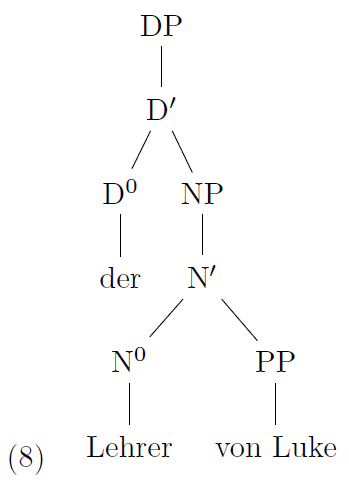
\includegraphics[width=.4\linewidth]{../../texfiles-beamer/tex-material/WissArb-latex/forest2}	
	\caption{without \ltxterm{linguistics}}
\end{figure}
\end{minipage}
%%
%%
\begin{minipage}[b]{.48\textwidth}
\begin{figure}
	\centering
	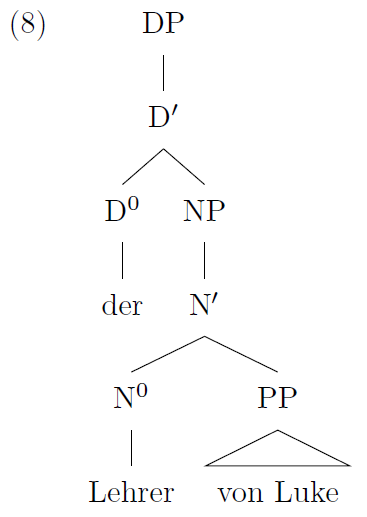
\includegraphics[width=.43\linewidth]{../../texfiles-beamer/tex-material/WissArb-latex/forest1}
	\caption{with \ltxterm{linguistics}}	
\end{figure}
\end{minipage}

\end{frame}


%%%%%%%%%%%%%%%%%%%%%%%%%%%%%%%%%%
\begin{frame}[fragile]
%\frametitle{Baumstrukturen}

\ltxpack{gb4e} re-defines some commands needed for \ltxpack{forest}. If you are using \ltxpack{gb4e}, you must load  \alert{\ltxpack{forest} first} and \alert{\ltxpack{gb4e} after}.

\begin{lstlisting}
\usepackage[linguistics]{forest}

\usepackage{gb4e}
\end{lstlisting}

\end{frame}


%%%%%%%%%%%%%%%%%%%%%%%%%%%%%%%%%%
%%%%%%%%%%%%%%%%%%%%%%%%%%%%%%%%%%
\subsection{forest syntax}
%\frame{
%	\frametitle{~}
%	\begin{multicols}{2}
%		\tableofcontents[currentsection,hideallsubsections]
%	\end{multicols}
%}
%%%%%%%%%%%%%%%%%%%%%%%%%%%%%%%%%%
%%%%%%%%%%%%%%%%%%%%%%%%%%%%%%%%%%

\begin{frame}[fragile]
\frametitle{forest syntax}

\begin{enumerate}
\item Use the \ltxterm{forest} \textbf{environment}.

\item Inside the \ltxterm{forest} environment write the \textbf{bracket notation} for your tree.

\item Do \textbf{not} use \textbf{empty lines}!
\end{enumerate}


\begin{lstlisting}
\begin{forest}
[S [NP] [VP]]
\end{forest}
\end{lstlisting}

\ea \begin{forest}
[S [NP] [VP]]
\end{forest}
\z 

\bigskip 

\begin{itemize}
	\item Practice the bracket notation: \url{http://ironcreek.net/phpsyntaxtree/}
\end{itemize}

\end{frame}


%%%%%%%%%%%%%%%%%%%%%%%%%%%%%%%%%%
\begin{frame}[fragile]
%\frametitle{Baumstrukturen}

For bigger trees, it is useful -- for the sake of clarity -- not to write the bracket notation linearly.

\begin{minipage}[t]{.48\textwidth}
\small	
\begin{lstlisting}
\begin{forest}
[S 
  [NP] 
  [VP
    [NP]
    [V$^{0}$]
  ]
]
\end{forest}
\end{lstlisting}

\vs

\begin{lstlisting}
\begin{forest}
[S [NP] [VP [NP] [V$^{0}$]]]
\end{forest}
\end{lstlisting}
\end{minipage}
%%
%%
\begin{minipage}[t]{.48\textwidth}
\begin{figure}

\centering
\begin{forest}
	[S 
	[NP] 
	[VP
	[NP]
	[V$^{0}$]
	]
	]
\end{forest}

\end{figure}

\end{minipage}

\end{frame}


%%%%%%%%%%%%%%%%%%%%%%%%%%%%%%%%%%
%%%%%%%%%%%%%%%%%%%%%%%%%%%%%%%%%%
\subsection{Trees in example environments}
%\frame{
%	\frametitle{~}
%	\begin{multicols}{2}
%		\tableofcontents[currentsection,hideallsubsections]
%	\end{multicols}
%}
%%%%%%%%%%%%%%%%%%%%%%%%%%%%%%%%%%
%%%%%%%%%%%%%%%%%%%%%%%%%%%%%%%%%%

\begin{frame}[fragile]
\frametitle{Trees in example environments}

\textbf{When using the option \ltxterm{linguistics}}, you can embed the tree in an example environment.


\begin{lstlisting}
\ea 
\begin{forest}
[S [NP] [VP]]
\end{forest}
\z
\end{lstlisting}

\ea 
\begin{forest}
	[S [NP] [VP]]
\end{forest}
\z 

\end{frame}


%%%%%%%%%%%%%%%%%%%%%%%%%%%%%%%%%%
%%%%%%%%%%%%%%%%%%%%%%%%%%%%%%%%%%
\subsection{Abbreviating nodes}
%\frame{
%	\frametitle{~}
%	\begin{multicols}{2}
%		\tableofcontents[currentsection,hideallsubsections]
%	\end{multicols}
%}
%%%%%%%%%%%%%%%%%%%%%%%%%%%%%%%%%%
%%%%%%%%%%%%%%%%%%%%%%%%%%%%%%%%%%

\begin{frame}[fragile]
\frametitle{Abbreviating nodes}


With the option \lstinline|roof|, you can abbreviate nodes.

\begin{multicols}{2}
	
\begin{lstlisting}
\ea 
\begin{forest}
[S 
  [NP [Colourless green ideas, roof]] 
  [VP [sleep furiously, roof]]
]
\end{forest}
\z 
\end{lstlisting}

\ea %
{\scriptsize %
\begin{forest}
	[S [NP [Colourless green ideas, roof]] [VP [sleep furiously, roof]]]
\end{forest}
}
\z 

\end{multicols}

\pause 

Take into account that options in \ltxpack{forest} (based on \ltxterm{TikZ}) are given by a \textbf{comma}. That means, you can use commas only when you \textbf{protect} them.

\begin{multicols}{2}
	
\begin{lstlisting}
\ea 
\begin{forest}
[S [NP [Noam{,} Irene{,} and Angelika, roof]] [VP [sleep, roof]]]
\end{forest}
\z 
\end{lstlisting}
	
	
\ea %
{\scriptsize %
	\begin{forest}
		[S 
		[NP [Noam{,} Irene{,} and Angelika, roof]] 
		[VP [sleep, roof]]
		]
	\end{forest}
}
\z 
\end{multicols}

\end{frame}


%%%%%%%%%%%%%%%%%%%%%%%%%%%%%%%%%%
%%%%%%%%%%%%%%%%%%%%%%%%%%%%%%%%%%
\subsection{Glossing or translating}
%\frame{
%	\frametitle{~}
%	\begin{multicols}{2}
%		\tableofcontents[currentsection,hideallsubsections]
%	\end{multicols}
%}
%%%%%%%%%%%%%%%%%%%%%%%%%%%%%%%%%%
%%%%%%%%%%%%%%%%%%%%%%%%%%%%%%%%%%

\begin{frame}[fragile]
\frametitle{Glossing or translating}


With \lstinline|\\|, you can add \textbf{glosses or translations} to your tree.


\begin{minipage}[t]{.48\textwidth}
\small	
\begin{lstlisting}
\begin{forest}
[S 
  [NP 
    [Peter \\ Peter \\ Pedro, roof]
  ] 
  [VP 
    [schläft tief. \\ sleeps deeply. \\ duerme profundamente, roof]
  ]
]
\end{forest}
\end{lstlisting}
\end{minipage}
%%
%%
\begin{minipage}[t]{.48\textwidth}

\begin{exe}
\ex 
\begin{forest}
[S [NP [Peter \\ Peter \\ Pedro, roof]] 
[VP [schläft tief. \\ 
sleeps deeply. \\ 
duerme profundamente, roof]]]
\end{forest}
\end{exe}
\end{minipage}

\end{frame}


%%%%%%%%%%%%%%%%%%%%%%%%%%%%%%%%%%
%%%%%%%%%%%%%%%%%%%%%%%%%%%%%%%%%%
\subsection{Sub- and superscript}
%\frame{
%	\frametitle{~}
%	\begin{multicols}{2}
%		\tableofcontents[currentsection,hideallsubsections]
%	\end{multicols}
%}
%%%%%%%%%%%%%%%%%%%%%%%%%%%%%%%%%%
%%%%%%%%%%%%%%%%%%%%%%%%%%%%%%%%%%

\begin{frame}[fragile]
\frametitle{Sub- and superscript}

The characters \lstinline|^| and \lstinline|_| are used in \textbf{math mode} for sub- and superscript, respectively. 
	
\begin{multicols}{2}

\begin{lstlisting}
$x^1$

$x_1$
\end{lstlisting}	

\ea $x^1$
\ex $x_1$
\z 

\end{multicols}

\pause 

The \textbf{default scope} of \lstinline|^| and \lstinline|_| is only one character (\ref{ex:SubSup1}), use \lstinline|{ }| to \textbf{expand} it, siehe (\ref{ex:SubSup2}). 


\begin{lstlisting}
\ea X$^1$ Y$^21$ X$_1$ Y$_21$ \label{ex:SubSup1}

\ex X$^{1}$ Y$^{21}$ X$_{1}$ Y$_{21}$ \label{ex:SubSup2}
\z 
\end{lstlisting}


\ea X$^1$ Y$^21$ X$_1$ Y$_21$ \label{ex:SubSup1}

\ex X$^{1}$ Y$^{21}$ X$_{1}$ Y$_{21}$ \label{ex:SubSup2}
\z 

\end{frame}


%%%%%%%%%%%%%%%%%%%%%%%%%%%%%%%%%%%
%\begin{frame}[fragile]
%%\frametitle{Baumstrukturen}
%
%\begin{itemize}
%\item Wie (\ref{ex:BspHochTief}) und (\ref{ex:BspKlammer}) zeigen, verhält sich \textbf{Text innerhalb vom Mathematikmodus} anders (kursiv ohne Spatien). 
%
%\item Um Text wiederzugeben verwenden Sie den Befehl \lstinline|\textrm{ }|, siehe Beispiel (\ref{ex:BspTxtRM}).
%\end{itemize}
%
%
%\begin{minipage}[t]{.45\textwidth}
%\scriptsize
%
%\begin{lstlisting}
%X$^{\textrm{Agens}}$ 
%
%Y$^{\textrm{Agens oder Patiens}}$
%
%X$_{\textrm{Agens}}$ 
%
%Y$_{\textrm{Agens oder Patiens}}$	
%\end{lstlisting}
%
%\end{minipage}
%%%
%%%
%\begin{minipage}[t]{.51\textwidth}
%
%\begin{exe}
%
%\exr{ex:BspHochTief}
%\begin{xlist}
%	\ex X$^Agens$ Y$^Agens oder Patiens$
%	\ex X$_Agens$ Y$_Agens oder Patiens$
%\end{xlist} 
%
%\exr{ex:BspKlammer}
%\begin{xlist}
%	\ex X$^{Agens}$ Y$^{Agens oder Patiens}$
%	\ex X$_{Agens}$ Y$_{Agens oder Patiens}$
%\end{xlist}
%
%\ex \label{ex:BspTxtRM}
%\begin{xlist}
%	\ex X$^{\textrm{Agens}}$ Y$^{\textrm{Agens oder Patiens}}$
%	\ex X$_{\textrm{Agens}}$ Y$_{\textrm{Agens oder Patiens}}$
%\end{xlist}
%
%\end{exe} 
%
%\end{minipage}
%
%\end{frame}


%%%%%%%%%%%%%%%%%%%%%%%%%%%%%%%%%%
\begin{frame}[fragile]
%\frametitle{Baumstrukturen}

Tree with sub- and superscripts

\begin{minipage}[t]{.48\textwidth}
\footnotesize	
\begin{lstlisting}
[CP
  [DP$_{21}$ [Peter \\ Peter, roof]]
  [C$^{\prime}$
    [C$^{0}$ [schläft$_{22}$ \\ sleeps]]
    [TP
      [$t_{21}$]
      [T$'$
        [VP
          [$t_{21}$]
          [V$^{\prime}$
            [V$^{0}$ [$t_{22}$]]
          ]
        ]
        [T$^{0}$ [$t_{22}$]]
      ]
    ]
  ]
]	
\end{lstlisting}
\end{minipage}
%%
%%
\begin{minipage}[t]{.48\textwidth}

\begin{figure}
\scriptsize
\centering 
\begin{forest}
[CP
[DP$_{21}$ [Peter \\ Peter, roof]]
[C$^{\prime}$
[C$^{0}$ [schläft$_{22}$ \\ sleeps]]
[TP
[$t_{21}$]
[T$'$
[VP
[$t_{21}$]
[V$^{\prime}$
[V$^{0}$ [$t_{22}$]]
]
]
[T$^{0}$ [$t_{22}$]]
]
]
]
]	
\end{forest}
\end{figure}
\end{minipage}

\end{frame}


%%%%%%%%%%%%%%%%%%%%%%%%%%%%%%%%%%
%%%%%%%%%%%%%%%%%%%%%%%%%%%%%%%%%%
\subsection{Arrows}
%\frame{
%	\frametitle{~}
%	\begin{multicols}{2}
%		\tableofcontents[currentsection,hideallsubsections]
%	\end{multicols}
%}
%%%%%%%%%%%%%%%%%%%%%%%%%%%%%%%%%%
%%%%%%%%%%%%%%%%%%%%%%%%%%%%%%%%%%

\begin{frame}[fragile]
\frametitle{Arrows}

Arrows/lines from node to node (\fe for movement, projection, etc.) can be drawn easily. 
	
Give the nodes a name (command: \lstinline|, name = |) and draw an arrow with the following command 
	
\begin{lstlisting}	
\draw[X] (Y) to[out=V, in=W] (Z);

\draw[->] (T10) to[out=south west, in=south west](T11);	
\end{lstlisting}
	
	\begin{itemize}
		\item \alert{X}: type of arrow/line (\lstinline|-> <- <-> -|)
		\item \alert{Y}: name of start node
		\item \alert{Z}: name of end node
		\item \alert{V}: start position of the node (\lstinline|south|/\lstinline|north| $+$ \lstinline|east|/\lstinline|west|)
		
		\item \alert{W}: end position of the node node (\lstinline|south|/\lstinline|north| $+$ \lstinline|east|/\lstinline|west|)
		
		\item \alert{;}: end of the command
	\end{itemize}
	
\end{frame}


%%%%%%%%%%%%%%%%%%%%%%%%%%%%%%%%%%
\begin{frame}[fragile]

%\begin{multicols}{2}

\begin{lstlisting}
[NP, name=N2
  [\textsc{Det} [die \\ the]]
  [N$'$, name=N1
    [N$^0$, name=N0 [Behandlung \\ treatment]]
    [NP [des Patienten \\ of the patient, roof]]
  ]
]
\draw[->,dashed] (N0) to[out=west,in=west] (N1);
\draw[->,dashed] (N1) to[out=east,in=east] (N2);
\end{lstlisting}

\begin{figure}[h]
\centering

\begin{forest}
[NP, name=N2
[\textsc{Det} [die \\ the]]
[N$'$, name=N1
[N$^0$, name=N0 [Behandlung \\ treatment]]
[NP [des Patienten \\ of the patient, roof]]
]
]
\draw[->,dashed] (N0) to[out=west,in=west] (N1);
\draw[->,dashed] (N1) to[out=east,in=east] (N2);
\end{forest}
\end{figure}

\nocite{MyP18b}
%\end{multicols}

\end{frame}

%%%%%%%%%%%%%%%%%%%%%%%%%%%%%%%%%%
\begin{frame}[fragile]
%\frametitle{Baumstrukturen}

\begin{minipage}[t]{.6\textwidth}
\scriptsize
%\tiny	
\begin{lstlisting}
[CP
  [DP$_{1}$, name=T12 [Peter, roof]]
  [C$^{\prime}$
    [C$^{0}$ [schläft$_{2}$, name=T22]]
    [TP
      [$t_{1}$, name=T11]
      [T$^{\prime}$
        [VP
          [$t_{1}$, name=T10]
          [V$^{\prime}$
            [V$^{0}$ [$t_{2}$, name=T20]]
          ]
        ]
        [T$^{0}$ [$t_{2}$, name=T21]]
      ]
    ]
  ]
]
\draw[->] (T10) 
to[out=south west, in=south west](T11);	
\draw[->] (T11) 
to[out=south west, in=south west](T12);
\end{lstlisting}
\end{minipage}
%%
%%
\begin{minipage}[t]{.38\textwidth}

\begin{figure}
	%\tiny
	\scriptsize
	\centering 
	\begin{forest}
		[CP
		[DP$_{1}$, name=T12 [Peter, roof]]
		[C$^{\prime}$
		[C$^{0}$ [schläft$_{2}$, name=T22]]
		[TP
		[$t_{1}$, name=T11]
		[T$^{\prime}$
		[VP
		[$t_{1}$, name=T10]
		[V$^{\prime}$
		[V$^{0}$ [$t_{2}$, name=T20]]
		]
		]
		[T$^{0}$ [$t_{2}$, name=T21]]
		]
		]
		]
		]
		\draw[->] (T10) to[out=south west, in=south west](T11);	
		\draw[->] (T11) to[out=south west, in=south west](T12);
	\end{forest}
\end{figure}
\end{minipage}

\end{frame}


%%%%%%%%%%%%%%%%%%%%%%%%%%%%%%%%%%
%%%%%%%%%%%%%%%%%%%%%%%%%%%%%%%%%%
\subsection{Marking nodes}
%\frame{
%	\frametitle{~}
%	\begin{multicols}{2}
%		\tableofcontents[currentsection,hideallsubsections]
%	\end{multicols}
%}
%%%%%%%%%%%%%%%%%%%%%%%%%%%%%%%%%%
%%%%%%%%%%%%%%%%%%%%%%%%%%%%%%%%%%

\begin{frame}[fragile]
\frametitle{Marking nodes}

Some options: 

\begin{itemize}
\item \lstinline|draw|: Viereck
\item \lstinline|circle, draw|: Kreis
\item \lstinline|red|: Knoten rot markieren
\item \lstinline|fill=X|: Knoten mit Farbe \emph{X} hinterlegen
\item \lstinline|circle, draw, fill=lightgray|: hellgrau hinterlegter Kreis 
\end{itemize}


%\end{frame}
%
%
%%%%%%%%%%%%%%%%%%%%%%%%%%%%%%%%%%%
%\begin{frame}[fragile]
%%\frametitle{Baumstrukturen}

\begin{minipage}[t]{.6\textwidth}
%\scriptsize
%\tiny	
\begin{lstlisting}
[S, draw
  [DP, circle, draw
    [Peter, roof]]
  [VP, draw, red 
    [DP, fill=blue 
      [einen Wagen, roof]]
    [V$^{0}$, circle, draw, fill=lightgray
      [kauft]]
  ]
]
\end{lstlisting}
\end{minipage}
%%
%%
\begin{minipage}[t]{.38\textwidth}

\begin{figure}
\centering 
\begin{forest}
[S, draw
[DP, circle, draw
[Peter, roof]
]
[VP, draw, red 
[DP, fill=blue 
[einen Wagen, roof]
]
[V$^{0}$, circle, draw, 
fill=lightgray
[kauft]
]
]
]
\end{forest}
\end{figure}
\end{minipage}

\end{frame}


%%%%%%%%%%%%%%%%%%%%%%%%%%%%%%%%%%
%%%%%%%%%%%%%%%%%%%%%%%%%%%%%%%%%%
\subsection{Further features}
%\frame{
%	\frametitle{~}
%	\begin{multicols}{2}
%		\tableofcontents[currentsection,hideallsubsections]
%	\end{multicols}
%}
%%%%%%%%%%%%%%%%%%%%%%%%%%%%%%%%%%
%%%%%%%%%%%%%%%%%%%%%%%%%%%%%%%%%%

\begin{frame}[fragile]
\frametitle{Further features}

\begin{itemize}
\item \ltxpack{forest} is a very powerful package. Check the package documentation \citep{Zivanovic17a} to see all of its benefits.

\item Check also the \emph{Quick start guide} for linguists \citep{VandenWyngaerd16a}.
\end{itemize}

\end{frame}


%%%%%%%%%%%%%%%%%%%%%%%%%%%%%%%%%
\begin{frame}[fragile]
\frametitle{Exercise}


Go to \url{https://github.com/langsci/latex4linguists/blob/master/4-1.md}\\
and\\
\url{https://github.com/langsci/latex4linguists/blob/master/4-2.md}
and follow the instructions of \textbf{all blocks} in your \texttt{.tex} file.

%Download the PDF \alert{\texttt{myDocument-EX4.pdf}} and replicate it with the commands you have already learnt. Follow the instructions in the last section and install the packages.

\end{frame}


%%%%%%%%%%%%%%%%%%%%%%%%%%%%%%%%%%%
%%%%%%%%%%%%%%%%%%%%%%%%%%%%%%%%%%%
%\section{XY}
%%\frame{
%%\begin{multicols}{2}
%%\frametitle{~}
%%	\tableofcontents[currentsection]
%%\end{multicols}
%%}
%%%%%%%%%%%%%%%%%%%%%%%%%%%%%%%%%%%
%
%\begin{frame}{XY}
%
%\begin{itemize}
%	\item XY
%\end{itemize}
%
%\end{frame}


%%%%%%%%%%%%%%%%%%%%%%%%%%%%%%%%%%%%
%%%%%%%%%%%%%%%%%%%%%%%%%%%%%%%%%%%%
%\iftoggle{handout}{
%%% BEGIN handout true
%
%%%%%%%%%%%%%%%%%%%%%%%%%%%%%%%%%%%%
%	
%%Test Toggle ON
%
%}
%%% END handout true 
%%% BEGIN handout false
%{
%%%%%%%%%%%%%%%%%%%%%%%%%%%%%%%%%%%%
%
%% Test Toggle OFF
%
%}%% END handout false
%%%%%%%%%%%%%%%%%%%%%%%%%%%%%%%%%%%%


%%%%%%%%%%%%%%%%%%%%%%%%%%%%%%%%%%%%%%%%%%%%%%%%%%%%
%%%                References                  
%%%%%%%%%%%%%%%%%%%%%%%%%%%%%%%%%%%%%%%%%%%%%%%%%%%% 

\appendix
\backupbegin


%%%%%%%%%%%%%%%%%%%%%%%%%%%%%%%%%%
%%%%%%%%%%%%%%%%%%%%%%%%%%%%%%%%%%
\section{Quellen}
%\frame{
%\begin{multicols}{2}
%\frametitle{~}
%	\tableofcontents[currentsection]
%\end{multicols}
%}
%%%%%%%%%%%%%%%%%%%%%%%%%%%%%%%%%%

\begin{frame}[allowframebreaks]
\frametitle{Quellen}

{\footnotesize
	
	\begin{itemize}
		\item Link: Bib\TeX\ -- Wikipedia (German)\\
		\url{https://de.wikipedia.org/wiki/BibTeX}\\
		{[}Zugriff: 23.10.2017]
		
		\item Link: Bib\TeX\ -- Wikipedia (English)\\
		\url{https://en.wikipedia.org/wiki/BibTeX}\\
		{[}Zugriff: 11.01.2019]
		
		\item Link: Bib\TeX .org\\
		\url{http://www.bibtex.org}\\
		{[}Zugriff: 23.10.2017]
		
		\item Link: Creating and Managing Bibliographies with Bib\TeX\ on Overleaf -- (Lian Tze Lim)\\
		\url{https://www.overleaf.com/blog/532-creating-and-managing-bibliographies-with-bibtex-on-overleaf}\\
		{[}Zugriff: 28.11.2017]
		
		\item Paket: \ltxpack{natbib} -- Flexible bibliography support.\\
		\url{https://ctan.org/pkg/natbib}\\
		{[}Zugriff: 23.10.2017]
		
		\item Twitter: \TeX\ tips\\
		\url{https://twitter.com/textip} \\
		{[}Zugriff: 10.04.2017]
		
		\item YouTube-Tutorial: \LaTeX\ Tutorial\\
		\url{https://www.youtube.com/channel/UCC-3dzj6dfbWwGzQzhkUS5A}\\
		{[}Zugriff: 23.10.2017]
		
		\item Link: Akzente und Sonderzeichen in \LaTeX .\\
		\url{https://de.wikibooks.org/wiki/LaTeX/_Akzente_und_Sonderzeichen}\\
		{[}Zugriff: 10.10.2017]

		\item Link: \LaTeX /Special Characters.\\
		\url{https://en.wikibooks.org/wiki/LaTeX/Special_Characters}\\
		{[}Zugriff: 02.01.2019]
		
		\item Link: CTAN -- The Comprehensive \TeX\ Archive Network .\\
		\url{http://www.ctan.org/}\\
		{[}Zugriff: 02.01.2019]
		
		\item Link: Type IPA phonetic symbols.\\
		\url{http://ipa.typeit.org/full/}\\
		{[}Access: 02/01/2019]
		
		\item Link: Language Science Press\\
		\url{www.langsci-press.org}\\
		{[}Access: 02/01/2019]		
		
		%%MATH MODE:
		\item Link: Detexify\\ 
		\url{http://detexify.kirelabs.org}\\
		{[}Zugriff: 08.12.2017]		
		
		\item Link: List of logic symbols -- Wikipedia\\ 
		\url{https://en.wikipedia.org/wiki/List_of_logic_symbols}\\
		{[}Zugriff: 08.12.2017]		
		
		\item Link: \LaTeX\ for Logicians:\\		
		\url{http://www.logicmatters.net/latex-for-logicians/}\\
		{[}Zugriff: 08.12.2017]				
		
		
		\item Link: The Great, Big List of \LaTeX\ Symbols \citep{Carlisle&Co01a}:\\
		\url{https://www.rpi.edu/dept/arc/training/latex/LaTeX_symbols.pdf}\\
		{[}Zugriff: 08.12.2017]		
		
		\item Link: The Comprehensive \LaTeX\ Symbol List -- Symbols accessible from \LaTeX\ \citep{Pakin17a}:\\
		\url{https://ctan.org/tex-archive/info/symbols/comprehensive/}\\
		{[}Zugriff: 08.12.2017]				

%		\item Grafik: Kontextuelle Bedeutung: Wrong Hands -- John Atkinson, \url{http://wronghands1.tumblr.com/post/157354512780} \\
%		{[}Zugriff: 23.01.2017]
%		
%		\item Grafik: Ludwig Wittgenstein: von Moritz Nähr -- Austrian National Library, Gemeinfrei, \url{https://commons.wikimedia.org/w/index.php?curid=46116699} \\
%		{[}Zugriff: 11.04.2017]	
%		
%		\item Grafik: Semantics -- the dark side: mdhk, \url{http://mdhk.tumblr.com/post/78033341047/yes} \\
%		{[}Zugriff: 29.07.2016]
%		
%		\item Grafik: Semantische Restriktionen: Linguist Llama, \url{http://lingllama.tumblr.com/post/14266418758/picture-background-8-piece-pie-style-color} \\
%		{[}Zugriff: 07.04.2014]
%		
%		\item Video: Trump vs.\ Truth: Last Week Tonight with John Oliver (HBO) \url{https://www.youtube.com/watch?v=xecEV4dSAXE} \\
%		{[}Zugriff: 12.04.2017]
		
	\end{itemize}
}

\end{frame}
%%%%%%%%%%%%%%%%%%%%%%%%%%%%%%%%%%


%%%%%%%%%%%%%%%%%%%%%%%%%%%%%%%%%%
%%%%%%%%%%%%%%%%%%%%%%%%%%%%%%%%%%
\section{Literatur}
%\frame{
%\begin{multicols}{2}
%\frametitle{~}
%	\tableofcontents[currentsection]
%\end{multicols}
%}
%%%%%%%%%%%%%%%%%%%%%%%%%%%%%%%%%%

\begin{frame}[allowframebreaks]
\frametitle{Literatur}

	%German
%	\bibliographystyle{../../texfiles-beamer/deChicagoMyP}

%	%English
%	\bibliographystyle{../../texfiles-beamer/enChicagoMyP} 
	\bibliographystyle{../../texfiles-beamer/unified} 

{\footnotesize
	\bibliography{../../texfiles-beamer/tex-literature}
}	
\end{frame}
%%%%%%%%%%%%%%%%%%%%%%%%%%%%%%%%%%

\backupend


\end{document}